\chapter{AgilePrimer} % Introduction chapter suppressed from the table of contents

\hypertarget{ux654fux6377ux662fux4ec0ux4e48}{%
\subsection{敏捷是什么}\label{ux654fux6377ux662fux4ec0ux4e48}}

\begin{itemize}
\tightlist
\item
  传统瀑布开发模式:依据范围(需求)估计时间和成本,然后监控
\item
  敏捷是反过来:固定每一个迭代时间段(例如两周),然后团队按自身能力估计本迭代可以开发多少内容(范围)
\end{itemize}

In a ``traditional'' world Time and Cost flex to meet Scope. In an Agile
world, Scope flexes to meet time and cost. Agile projects are never
late! But they may not deliver what you need the first time.\\

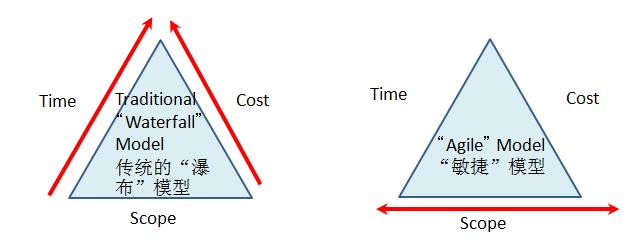
\includegraphics[width=10cm]{P9.jpg}

传统瀑布型项目,
按需求调研写成软件需求规格书,与客户确认后,做个详细计划(如,3到6个月)。但如果在过程中需求有变化,会导致后面无法按原计划开发,最常见的问题就是:项目结束时间还是不动,按本来时间交付,导致项目就要把后面的开发和测试时间压缩。我看过有些项目就是有这种原因,导致本来两周的系统测试被压缩到一两天,严重影响项目质量。\\
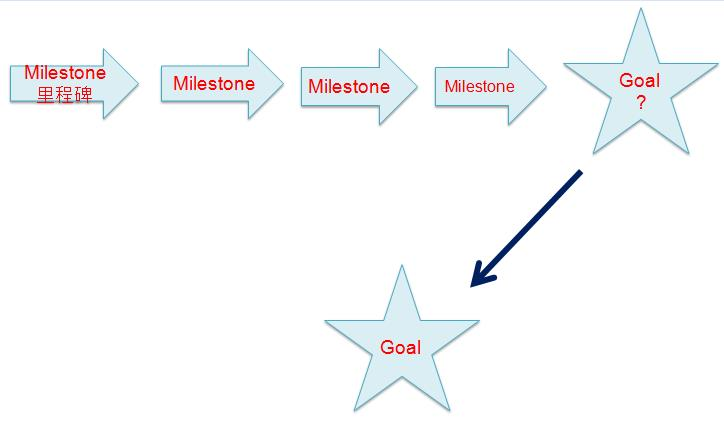
\includegraphics[width=10cm]{P10.jpg}

传统瀑布模式都会像上图,先有需求文档,然后设计、测试等,按各阶段,做出最终产品。

在敏捷开发,会把整个开发分成冲刺,把所有要做的按优先级逐步开发。这个就可以减少瀑布模式难以应付需求变更的问题。

\begin{itemize}
\tightlist
\item
  精益的概念,争取在每一个迭代,做出测试好可运行的软件,并演示给客户,获取反馈。
\end{itemize}

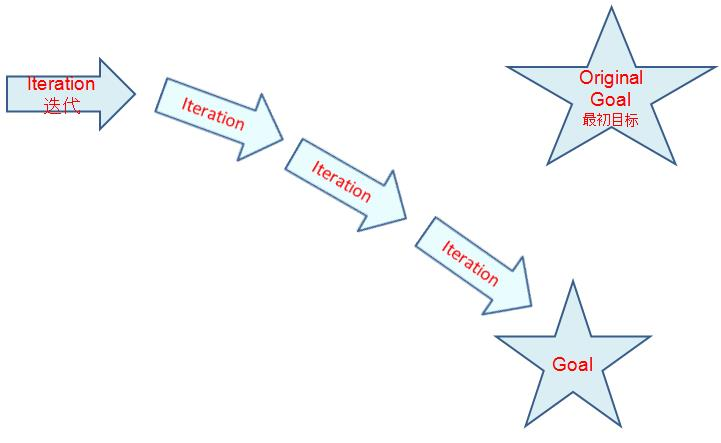
\includegraphics[width=10cm]{P11.jpg}

\hypertarget{ux6280ux5de7-agile-techniques}{%
\subsection{技巧 Agile Techniques}\label{ux6280ux5de7-agile-techniques}}

\begin{itemize}
\tightlist
\item
  增量设计 Incremental design and documents
\item
  测试驱动开发 Test-based design
\item
  每日站会 Daily Standup meeting
\item
  冲刺展示 Sprint demo
\item
  冲刺回顾/复盘 Sprint retrospective
\item
  重构 Refactoring
\end{itemize}

\hypertarget{ux654fux6377ux5f00ux53d1ux6b65ux9aa4}{%
\subsection{敏捷开发步骤}\label{ux654fux6377ux5f00ux53d1ux6b65ux9aa4}}

\begin{itemize}
\tightlist
\item
  以scrum为例子,一个迭代会包括从需求来的产品Backlog,然后每个团队团队按照优先级算当前迭代的冲刺Backlog。每天利用站立会议管理问题和风险。每个层次都以最后展示给客户可执行的一个软件作为完成标准,这个叫冲刺展示,展示后也需要有团队的回顾、复盘,改进下一个冲刺。\\
\item
  敏捷很注重代码的质量,不会花精力在一些无用的文档上面,但会注重测试驱动开发、重构等方法,确保软件开发质量;也重视给团队反馈,鼓励用白板、墙上贴纸等方式,让大家知道现在的进展情况。
\end{itemize}

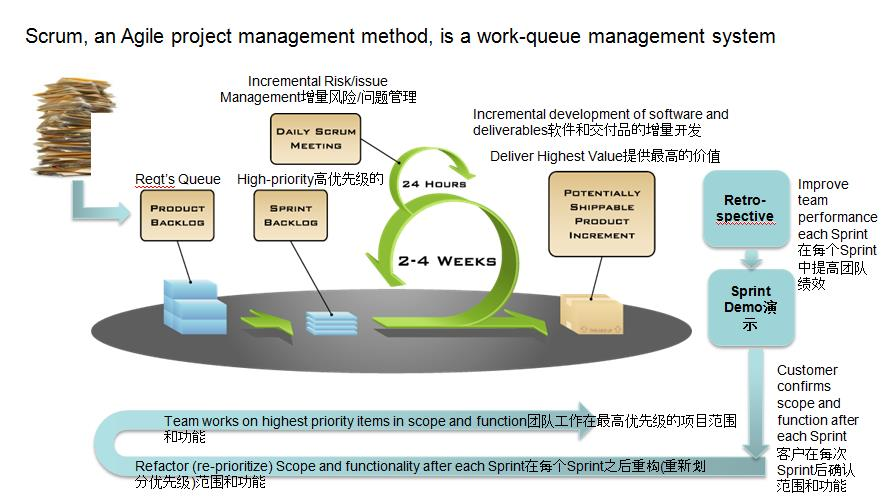
\includegraphics[width=10cm]{0A_Agile_stories_p13.jpg}

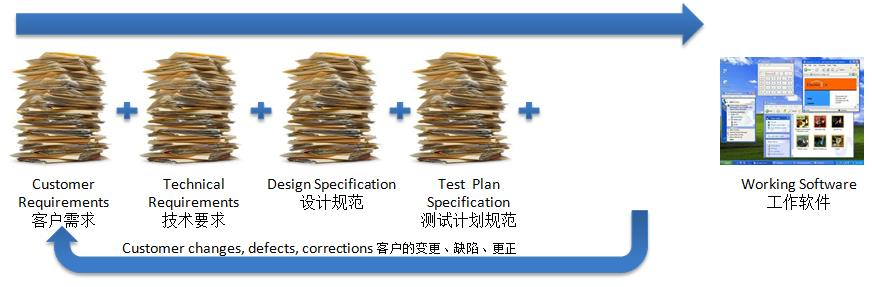
\includegraphics[width=10cm]{P12_1.jpg}

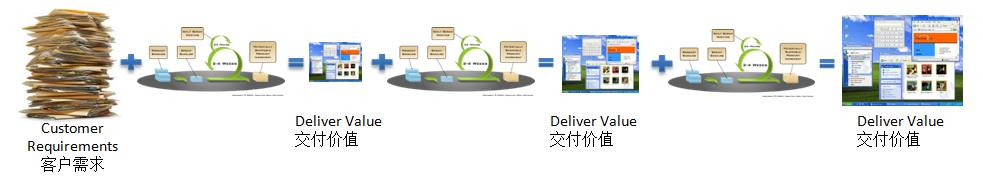
\includegraphics[width=10cm]{P12_2.jpg}

\hypertarget{ux6210ux529fux8981ux7d20}{%
\subsection{成功要素}\label{ux6210ux529fux8981ux7d20}}

\begin{itemize}
\tightlist
\item
  是否内部人员开发 -\/-
  如果都分包出去的话,难以利用敏捷,因为他们跟公司只有外包合同关系,导致这种敏捷难以用于他们外包
\item
  团队不能分散,也不能太大
\item
  团队的能力 -\/- 如果都是毕业生,就难以启动敏捷项目了
\item
  客户参与很重要 -\/-
  需要每2周给开发反馈,防止几个月后才发现不满足客户想法
\item
  依赖开发团队与产品经理(Product owner) 合作,使软件开发集合产品的理念
\end{itemize}

不是所有项目都适合用敏捷,以下问题可以帮我们判断:

\begin{enumerate}
\tightlist
\item
  所有的功能是否都可以容易在用户界面看得到?
\item
  所有的最终用户都可以明确识别出来,方便功能的确认;
\item
  是否很多复杂算法?这种的话可能就不太合适;
\item
  是否可以细分到子系统模块?如果太大的话也不适合做冲刺迭代,团队不能太大;
\item
  项目是否有时间限制?有的话就更合适用迭代定期来做;
\item
  需求是否没有详细的内容,只是一个概括,后面容易不断的演化、变化,这种的话就呃比较合适做敏捷开发,避免前面说到的,在需求慢慢演化中导致大量的变更。\\
\end{enumerate}

\hypertarget{ux654fux6377ux5ba3ux8a00-the-agile-manifesto}{%
\subsection{敏捷宣言 The Agile
Manifesto*}\label{ux654fux6377ux5ba3ux8a00-the-agile-manifesto}}

2000年,17位敏捷大师在盐湖城开会,得出以下大家都赞同的敏捷原则:

\begin{itemize}
\tightlist
\item
  我们一直探索,也帮助他人,发现软件开发更好的方法。
\end{itemize}

We are uncovering better ways of developing software by doing it and
helping others do it.\\

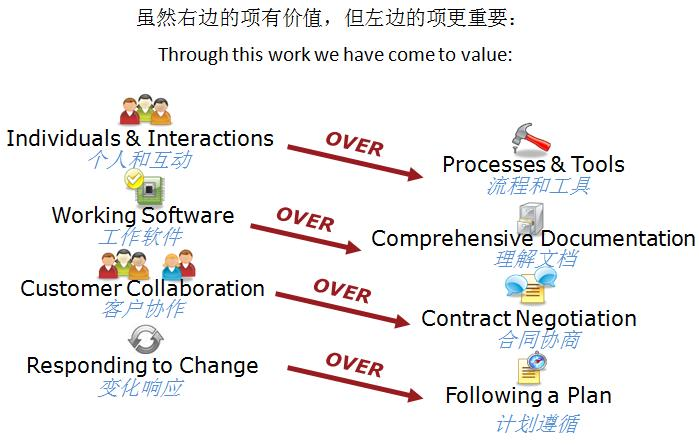
\includegraphics[width=10cm]{P6The_Agile_Manifesto.jpg}

\hypertarget{ux6761-ux539fux5219}{%
\subsection{12条 原则}\label{ux6761-ux539fux5219}}

\begin{enumerate}
\tightlist
\item
  最优先要做的是尽早、持续地交付有价值的软件,让客户满意。(Our highest
  priority is to satisfy the customer through early and continuous
  delivery of valuable software.)
\item
  欣然面对需求变化,即使在开发后期。敏捷过程利用变化为客户维持竞争的优势。(Welcome
  changing requirements, even late in development. Agile processes
  harness change for the customer's competitive advantage.)
\item
  频繁地交付可工作的软件,从数周到数月,交付周期越短越好。(Deliver
  working software frequently, from a couple of weeks to a couple of
  months, with a preference to the shorter timescale.)
\item
  在团队内外,面对面交谈是最有效,也是最高效的沟通方式。(Business
  people and developers must work together daily throughout the
  project.)
\item
  在整个项目过程中,业务人员必须和开发人员每天都在一起工作。(Build
  projects around motivated individuals. Give them the environment and
  support they need, and trust them to get the job done.)
\item
  以受激励的个体为核心构建项目。为他们提供所需的环境和支持,相信他们可以把工作做好。(The
  most efficient and effective method of conveying information to and
  within a development team is face-to-face conversation.)
\item
  可工作的软件是衡量进度的首要标准。(Working software is the primary
  measure of progress.)
\item
  敏捷过程倡导可持续开发。(Agile processes promote sustainable
  development. The sponsors, developers, and users should be able to
  maintain a constant pace indefinitely.)
\item
  坚持不懈的追求技术卓越和良好的设计,以此增强敏捷的能力。(Continuous
  attention to technical excellence and good design enhances agility.)
\item
  简单是尽最大可能减少不必要工作的艺术,是敏捷的根本。(Simplicity-\/-the
  art of maximizing the amount of work not done is essential.)
\item
  最好的架构、需求和设计来自自组织的团队。(The best architectures,
  requirements, and designs emerge from self-organizing teams.)
\item
  团队定期反思如何提升效率,并依此自我调整。(At regular intervals, the
  team reflects on how to become more effective, then tunes and adjusts
  its behavior accordingly.)
\end{enumerate}


